\begin{flushleft}
    \huge
    \textbf{4. Testing}
    \vspace{0.1cm}
    
    \Large{\textbf{4.1 Testing Table}}
    \vspace{0.5cm}
    
    \large
    As part of testing my NEA, I identified the key areas of my project which needed testing.
    My testing targets these areas from different angles to ensure they work correctly. 
    These areas are:
    \begin{enumerate}
        \item User Input and Program Output
            \begin{enumerate}
                \item Parameter Loading
                \item Neural Network Loading
                \item Graphical Output
                \item Console Output
            \end{enumerate}
        \item Matrix Implementation
            \begin{enumerate}
                \item Constructor Cases
                \item Matrix Operations
                \item Thrown Exceptions
            \end{enumerate}
        \item Deep Q Learning Algorithm
            \begin{enumerate}
                \item Forward Propagation
                \item Loss Function
                \item Back Propagation
                \item Double Ended Queue Data Type
            \end{enumerate}
        \item Data Logger
            \begin{enumerate}
                \item Data Structure Matching
                \item Heap Data Structure
                \item Heap Sort Implementation
            \end{enumerate}
        \item Simulation
            \begin{enumerate}
                \item Generation of 2d Terrain
                \item Continuity of Generation
                \item ML Agent
                \item Reward Methods
            \end{enumerate}
    \end{enumerate}
    
    \pagebreak
    
    \begin{center}
        \large
        \textbf{Below is included an NEA Testing video used for some parts of Testing Evidence}
        
        \vspace{0.2cm}
        
        \Large
        \textit{https://thisisalink.com/youtotallybelieveme/}
    \end{center}
    
    \vspace{1cm}
    \large{\textbf{1. User Input and Program Output}}
    \vspace{0.5cm}
    
    \normalsize
    \begin{longtable}{| C{0.6cm} | C{3cm} | C{4cm} | C{5cm} | L{1cm} | L{1.4cm} |}
        \hline
        {\footnotesize Test No.} & Test Name & Input Data / Description & Expected Output & Pass / Fail & Testing Evidence \\
        \hline\hline
        \rn & Loading Parameters File & Input "Default.json" file which contains the loadable values & Loads parameters into the 
        Parameters Dictionary variable & Pass & 1.1 \\ 
        \hline
        \rn & Parameters within range & Input Loaded Parameters Dictionary & Prints to console "Parameters within Specified Ranges" & Pass & 1.2 \\
        \hline
        \rn & Below Range Parameter & Input "Default.json" file with a below range parameters & Raises an exception detailing the Parameter, 
        Value of Parameters, and the given Range Required & Pass & 1.3 \\
        \hline
        \rn & Above Range Parameter & Input "Default.json" file with an above range parameters & Raises an exception detailing the Parameter, 
        Value of Parameters, and the given Range Required  & Pass & 1.4 \\
        \hline
        \rn & Network Saved Data Loading & When Prompted to load network data type "Y", and type the file name of network data to load & Network 
        Data is loaded successfully, training position stored & Pass & 1.5 \\
        \hline
        \rn & Window Opening & Run Program, enter setup info as normal & Window opens and is of the correct size/resolution & Pass & 1.6 \\
        \hline
        \rn & Window Displays correct debug information & Run Program, enter setup info as normal, with "Debug" = 1 in parameters file & Debug 
        Layer output info displayed on Right side of Window & Pass & 1.7 \\
        \hline
        \rn & Agent is displayed & Run Program, enter setup info as normal & Orange square displayed on screen & Pass & 1.8 \\
        \hline
        \rn & Enemies are displayed & Run Program, enter setup info as normal, with "StartEnemyCount" $\greatereq$ 1  & Red Square/s are displayed 
        on Screen & Pass & 1.9 \\
        \hline
        \rn & Console Messages Output & Run Program, enter setup info as normal & Console Messages Outputted per 100 Steps & Pass & 1.10 \\
        \hline
    \end{longtable}
    
    \vspace{1cm}
    \large{\textbf{2. Matrix Implementation}}
    \vspace{0.5cm}
    
    \normalsize
    \begin{longtable}{| C{0.6cm} | C{3cm} | C{4cm} | C{5cm} | L{1cm} | L{1cm} |}
        \hline
        {\footnotesize Test No.} & Test Name & Input Data / Description & Expected Output & Pass / Fail & Testing Evidence \\
        \hline\hline
        \rn & Create Matrix with Tuple & A Tuple for the order of the Matrix & Matrix is created with an order the same as the Tuple & - & - \\
        \hline
        \rn & Create Matrix with 2d List & A 2d List, where the parent list holds a list for every row, each "row list" is of the same length & Matrix is created with the same values as the 2d List & - & - \\
        \hline
        \rn & Create Vector with List & A 1d List of any Values  & Vector is created with the same values as the List & - & - \\
        \hline
        \rn & Print Matrix to Console & A valid Matrix of any size & Matrix Prints to the console with the correct formatting & - & - \\
        \hline
        \rn & Create Randomised Matrix & A Tuple for the order of the Matrix, and the the keyargument random=True & Matrix is created with randomised values between -0.5 and 0.5 & - & - \\
        \hline
        \rn & Create Identity Matrix & A Tuple for the order of the Matrix, and the the keyargument identity=True & Matrix is created with all 0's and 1's down the diagonal & - & - \\
        \hline
        \rn & Matrix Addition Calculation & Two Matrices of the same order & Matrix Addition is performed to create a new Matrix with the added values & - & - \\
        \hline
        \rn & Matrix Subtraction Calculation & Two Matrices of the same order & Matrix Subtraction is performed to create a new Matrix with the subtracted values & - & - \\
        \hline
        \rn & Matrix Multiplication Calculation & Two Matrices where Width of $M1$ is equal to the height of $M2$ & Matrix Multiplication is performed to create a new Matrix with the multiplied values & - & - \\
        \hline
        \rn & Matrix Scalar Multiplication Calculation & A $float/int$ as the scalar and any size Matrix & Matrix Scalar Multiplication is performed to create a new Matrix with the multiplied values & - & - \\
        \hline
        \rn & Vector Hadamard Product Calculation & Two Vectors with the same Order & Vector Hadamard Product is performed to create a new Vector with the multiplied values & - & - \\
        \hline
        \rn & Matrix Power Calulation & A Square Matrix with values stored in it & Matrix to the Power of is performed to create a new Matrix with the correct values & - & - \\
        \hline
        \rn & Matrix Transpose Calculation & A Matrix with values stored in it & New Matrix is created with values flipped across the diagonal & - & - \\
        \hline
        \rn & Matrix Select Column & A Matrix with values stored in it & Selects the indexed Column from the Matrix, returning as a list & - & - \\
        \hline
        \rn & Matrix Select Row & A Matrix with values stored in it & Selects the indexed Row from the Matrix, returning as a list & - & - \\
        \hline
        \rn & Vector Max in Vector & A Vector & Returns Largest value in Vector & - & - \\
        \hline
        \rn & Matrix Clear & A Matrix with values stored in it & Clears Matrix of any values & - & - \\
        \hline
        \rn & Combine Vectors & List of Vectors of the same Order & Combines the list of Vectors into a Matrix & - & - \\
        \hline
        \rn & Matrix Sum & - & Sums all values in the Matrix returning a $float/int$ & - & - \\
        \hline
        \rn & Randomised Matrix Constructor Tests & Generator Constructor Parameters randomnly for 10000 Tests & All Tests Should produce a valid Matrix & Pass & 2.16 \\
        \hline
        \rn & Randomised Constructor Exception Tests & Generate Random Data to cause Exceptions within the Constructor for 10000 Tests & All Tests should 
        trigger the Targetted Exception for that test & Pass & 2.17 \\
        \hline
        \rn & Randomised Operator Tests & Generator Random Data to test the Operator Methods for 10000 Tests & All Tests should produce the correct result & Pass & 2.18 \\
        \hline
        \rn & Randomised Operator Exception Tests & Generate Random Data to cause Exceptions within the Operators for 10000 Tests & All Tests should 
        trigger the Targetted Exception for that test & Pass & 2.19 \\
        \hline
    \end{longtable}

    \vspace{1cm}
    \large{\textbf{3. Deep Q Learning Algorithm}}
    \vspace{0.5cm}
    
    \small
    \begin{longtable}{| C{0.6cm} | C{3cm} | C{4cm} | C{5cm} | L{1cm} | L{1cm} |}
    \hline
    {\footnotesize Test No.} & Test Name & Input Data / Description & Expected Output & Pass / Fail & Testing Evidence \\
        \hline\hline
        \rn & Networks are Created & Run Program, enter setup info, denying the loading of weights & A Dual Neural Network is created after Program Start & - & - \\
        \hline
        \rn & Networks conforms to Parameters & Run Program, enter setup info, denying the loading of weights & The created Dual Neural Network conforms to the specified structure 
        in the parameter "DeepQLearningLayers" & - & - \\
        \hline
        \rn & Forward Propagation Test & Where L is the Current Layer, Forward Propagation requires: $Output Vector^{L-1}, Weight Matrix^{L-1}, Bias Vector^{L}$ 
        & The output of the Layer & - & - \\
        \hline
        \rn & Forward Propagation Multi Layer Test & Same as Entry Above & - & - & - \\
        \hline
        \rn & Loss Function Bellman Equation & - & - & - & - \\
        \hline
        \rn & Back Propagation Unit Test & - & - & - & - \\
        \hline
        \rn & Back Propagation Multi Layer Unit Test & - & - & - & - \\
        \hline
        \rn & Deque Push Front & A value to push to the Deque & Item is pushed to front of Deque & - & 3.8 \\
        \hline
        \rn & Deque First/Last & Call the .First() or .Last() Method for a Deque Object & Returns item at Front/Last index of Deque & - & - \\
        \hline
        \rn & Deque Sample N Ammount of Items & Call the .Sample(int N) Method, with a parameter of N items, for a Deque Object & Returns N number of random 
        samples from Deque & - & - \\
        \hline
        \rn & Experience Replay Sampling & - & Back Propagation is performed on the sampled Deque Items & - & - \\
        \hline
        \rn & Activation Outputs Unit Test & Input Value Vector to the Activation Function & Returns a Vector of values, where the Activation has been 
        applied to them & - & - \\
        \hline
        \rn & Activation Derivatives Output Unit Test & Input Value Vector to the Activation Derivative Function & Returns a Vector of values, where the 
        Activation Deivative has been applied to them & - & - \\
        \hline
    \end{longtable}

    \vspace{1cm}
    \large{\textbf{4. Data Logger}}
    \vspace{0.5cm}
    
    \normalsize
    \begin{longtable}{| C{0.6cm} | C{3cm} | C{4cm} | C{5cm} | L{1cm} | L{1cm} |}
    \hline
    {\footnotesize Test No.} & Test Name & Input Data / Description & Expected Output & Pass / Fail & Testing Evidence \\
        \hline\hline
        \rn & Heap Sort Decending & A randomnly generated input list & Sorts the list of items into Descending order & Pass & 4.1 \\
        \hline
        \rn & Add Point & A Data Point matching the data structure of the DataCollector & Point is added to Data Points list & Pass & 4.2 \\
        \hline
        \rn & Match Data Struture with Single & Data Structure contrains an index with a Single-Typed 
        definition & No error thrown & Pass & 4.3 \\
        \hline
        \rn & Match Data Struture with Multi-Typed & Data Structure contrains an index with a Multi-Typed
        definition & No error thrown & Pass & 4.4 \\
        \hline
        \rn & Match Data Struture with List-Typed & Data Structure contrains an index with a List-Typed 
        definition & No error thrown & Pass & 4.5 \\
        \hline
        \rn & Match Data Structure Error & Try match point with structure which does not match & Error is thrown with correct info & Pass & 4.6 \\
        \hline
        \rn & Select Query & Select from DataLogger with an Index and Search Contents & Returns a list of the selected column where the Search Contents Matches & Pass & 4.7 \\
        \hline
        \rn & Save Data Points & Invoke Save method on DataLogger Object & Saves Data Points to specified File & Pass & 4.8 \\
        \hline
        \rn & Load Data Points & Invoke Load method on DataLogger Object & Loads Data Points from specified File & Pass & 4.9 \\
        \hline
    \end{longtable}

    \vspace{1cm}
    \large{\textbf{5. Simulation}}
    \vspace{0.5cm}
    
    \normalsize
    \begin{longtable}{| C{0.6cm} | C{3cm} | C{4cm} | C{5cm} | L{1cm} | L{1cm} |}
    \hline
    {\footnotesize Test No.} & Test Name & Input Data / Description & Expected Output & Pass / Fail & Testing Evidence \\
        \hline\hline
        \rn & Creation of Agent & Run progam as normal & Agent is created as an instance of the Agent Class & - & - \\
        \hline
        \rn & Creation of Enemies & Run program as normal with the "StartEnemyCount" Parameter $\greatereq 1$ & Up to the ammount of specified Enemies are created & - & - \\
        \hline
        \rn & Enemies Pathfind towards Agent & Run program as normal with "StartEnemyCount" Parameter $\greatereq 1$ & The spawned enemies pathfind towards the agnet 
        using the defined pathfinding algorithm & - & - \\
        \hline
        \rn & Getting Tile Data & Call .GetTileVector(worldMap, enemyList[]) with arguments for worldMap and the list of current Enemies & Returns a Vector of the 
        surrounding tile objects & - & - \\
        \hline
        \rn & Convert Tile Data & Call .TileVectorPostProcess(tileVec) with argument of the result from the Test Above & Converts Tile Data into two vectors, Grayscale 
        Colour and Tile Type & - & - \\
        \hline
        \rn & Reward System Test Basic Reward & - & Expected reward is given to agent & - & - \\
        \hline
        \rn & Reward System Test Complex Reward & - & Expected reward is given to agent & - & - \\
        \hline
        \rn & World Generates to an Acceptable Standard & Run program as normal & Generates 2d Terrain which roughly looks realistic & - & - \\
        \hline
        \rn & World Generation Conforms to Parameters & Utilise inputted parameters to identify the effect they have on the world Generation & Terrain changes depending on inputting Parameters & - & - \\
        \hline
        \rn & Perlin Noise retains Continuity & Generate two worlds with the same seed & Perlin Noise returns same value when using the same seed twice & - & - \\
        \hline
    \end{longtable}
    
    \pagebreak
    \vspace{1cm}
    \Large{\textbf{4.2 Testing Evidence}}
    
    \vspace{0.5cm}

    \setcounter{magicrownumbers}{0}
    \normalsize
    \begin{center}
        {\large Evidence 1.\rn }\\ 
        \vspace{0.3cm}
        The .json file which is being loaded \\
        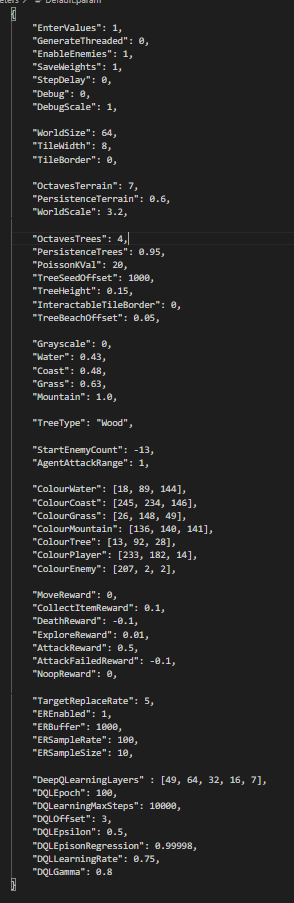
\includegraphics[width=6cm]{Images/Testing/T1.1.1.PNG} \\
        Printing the loaded Json File to console to Console to check the values match\\
        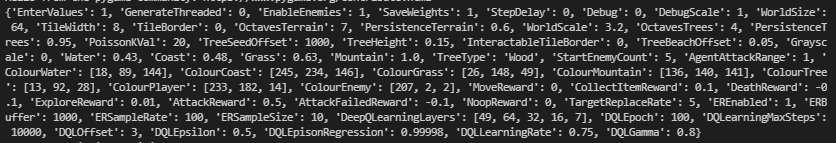
\includegraphics[width=16cm]{Images/Testing/T1.1.2.PNG} \\
        \vspace{1cm}

        {\large Evidence 1.\rn } \\ 
        \vspace{0.3cm}
        Console Output when parameters are within specified ranges \\
        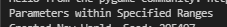
\includegraphics[width=6cm]{Images/Testing/T1.2.1.PNG} \\
        A Screenshot of the .json file where the Ranges are defined \\
        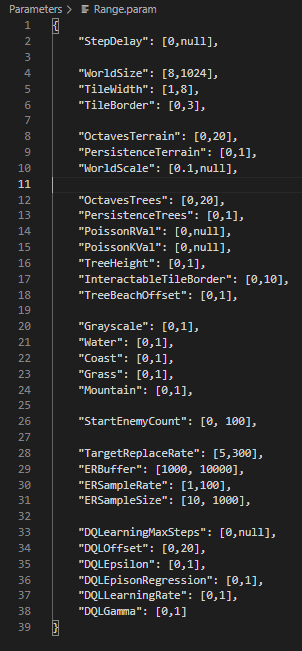
\includegraphics[width=6cm]{Images/Testing/T1.2.2.PNG}
        \vspace{1cm}

        {\large Evidence 1.\rn } \\ 
        \vspace{0.3cm}
        The given out of range parameter - subceeding \\
        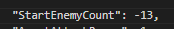
\includegraphics[width=6cm]{Images/Testing/T1.3.1.PNG} \\
        The specified range it should be within \\
        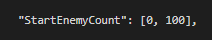
\includegraphics[width=6cm]{Images/Testing/T1.3.2.PNG} \\
        The Exception thrown when the program is run \\
        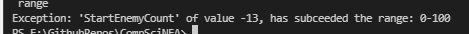
\includegraphics[width=12cm]{Images/Testing/T1.3.3.PNG} \\
        \vspace{1cm}

        {\large Evidence 1.\rn }\\ 
        \vspace{0.3cm}
        The given out of range parameter - exceeding \\
        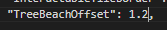
\includegraphics[width=6cm]{Images/Testing/T1.4.1.PNG} \\
        The specified range it should be within \\
        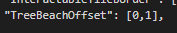
\includegraphics[width=6cm]{Images/Testing/T1.4.2.PNG} \\
        The Exception thrown when the program is run \\
        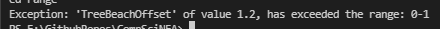
\includegraphics[width=12cm]{Images/Testing/T1.4.3.PNG} \\
        \vspace{1cm}

        {\large Evidence 1.\rn }\\ 
        \vspace{0.3cm}
        The Console prompt if the user wants to load Network Weights \\
        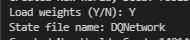
\includegraphics[width=6cm]{Images/Testing/T1.5.1.PNG} \\
        The file the program is loading \\
        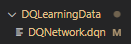
\includegraphics[width=4cm]{Images/Testing/T1.5.2.PNG} \\
        The testing step resumes at 400, underlined in Red \\
        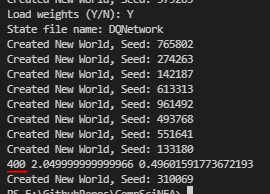
\includegraphics[width=6cm]{Images/Testing/T1.5.3.PNG}
        \vspace{1cm}

        {\large Evidence 1.\rn } \\ 
        \vspace{0.3cm}
        The width/height of the window\\
        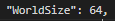
\includegraphics[width=4cm]{Images/Testing/T1.6.1.PNG} \\
        The opened window, it is 64 wide and 64 tall \\
        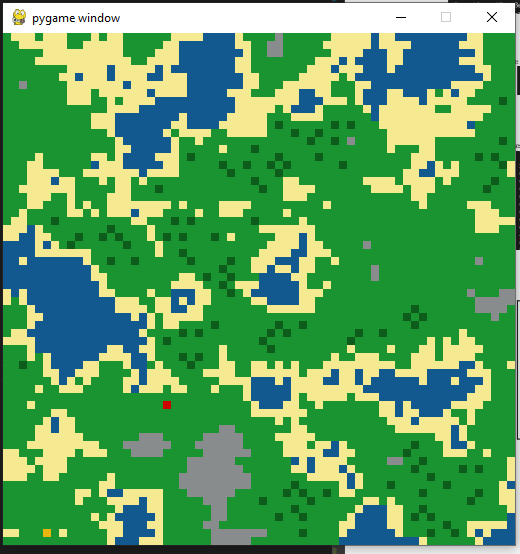
\includegraphics[width=8cm]{Images/Testing/T1.6.2.PNG}
        \vspace{1cm}

        {\large Evidence 1.\rn } \\ 
        \vspace{0.3cm}
        Debug being set to 1 in the parameters file \\
        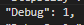
\includegraphics[width=4cm]{Images/Testing/T1.7.1.PNG} \\
        The displayed debug information to the right of the Window \\
        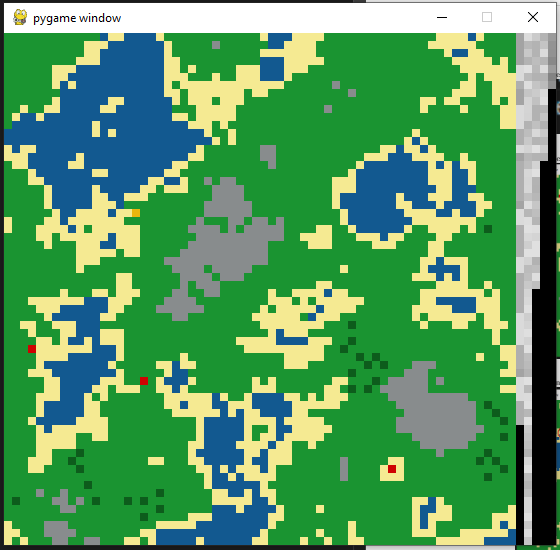
\includegraphics[width=8cm]{Images/Testing/T1.7.2.PNG} \\
        \vspace{1cm}

        {\large Evidence 1.\rn } \\ 
        \vspace{0.3cm}
        The opened window, with the agent circled \\
        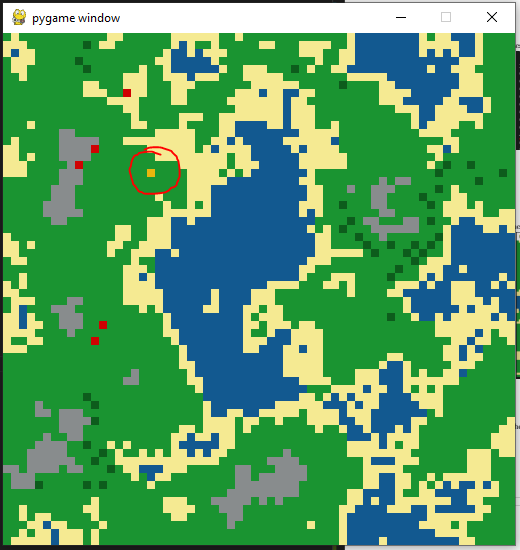
\includegraphics[width=8cm]{Images/Testing/T1.8.1.PNG} \\
        \vspace{1cm}

        {\large Evidence 1.\rn } \\ 
        \vspace{0.3cm}
        The opened window, with the enemies circled \\
        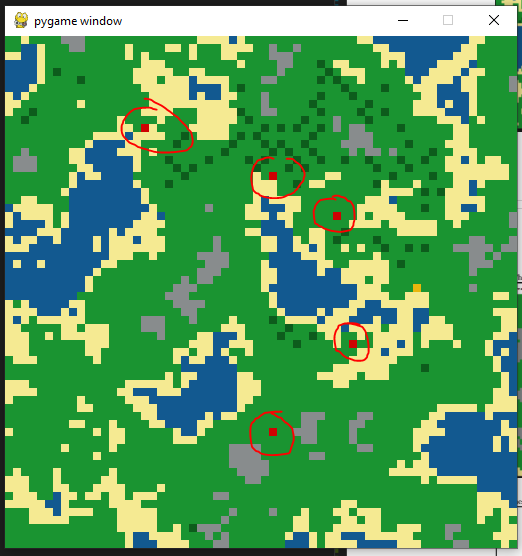
\includegraphics[width=8cm]{Images/Testing/T1.9.1.PNG} \\
        \vspace{1cm}

        {\large Evidence 1.\rn } \\ 
        \vspace{0.3cm}
        The correctly displayed console outputs \\
        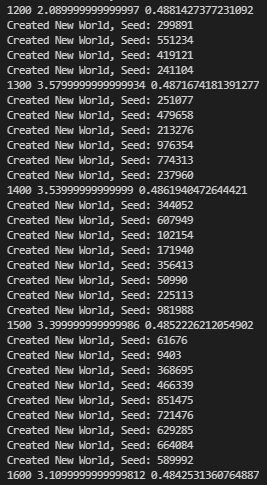
\includegraphics[width=8cm]{Images/Testing/T1.10.1.PNG} \\
    \end{center}

    \setcounter{magicrownumbers}{0}
    \begin{center}
        {\large Evidence 2.\rn } \\ 
        \vspace{0.3cm}
        Console Output, all Tests have passed with no failures \\
        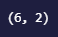
\includegraphics[width=4cm]{Images/Testing/T2.16.1.PNG} \\
        \vspace{1cm}

        {\large Evidence 2.\rn } \\ 
        \vspace{0.3cm}
        Console Output, all Tests have passed with no failures \\
        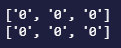
\includegraphics[width=4cm]{Images/Testing/T2.17.1.PNG} \\
        \vspace{1cm}

        {\large Evidence 2.\rn } \\ 
        \vspace{0.3cm}
        Console Output, all Tests have passed with no failures \\
        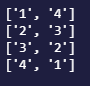
\includegraphics[width=4cm]{Images/Testing/T2.18.1.PNG} \\
        \vspace{1cm}

        {\large Evidence 2.\rn } \\ 
        \vspace{0.3cm}
        Console Output, all Tests have passed with no failures \\
        
\includegraphics[width=4cm]{Images/Testing/T2.19.1.PNG} \\
        \vspace{1cm}
    \end{center}

    \setcounter{magicrownumbers}{0}
    \begin{center}
        {\large Evidence 3.\rn } \\ 
        \vspace{0.3cm}
        \vspace{1cm}
        
        {\large Evidence 3.\rn } \\ 
        \vspace{0.3cm}
        \vspace{1cm}

        {\large Evidence 3.\rn } \\ 
        \vspace{0.3cm}
        \vspace{1cm}

        {\large Evidence 3.\rn } \\ 
        \vspace{0.3cm}
        \vspace{1cm}

        {\large Evidence 3.\rn } \\ 
        \vspace{0.3cm}
        \vspace{1cm}

        {\large Evidence 3.\rn } \\ 
        \vspace{0.3cm}
        \vspace{1cm}

        {\large Evidence 3.\rn } \\ 
        \vspace{0.3cm}
        \vspace{1cm}

        {\large Evidence 3.\rn } \\ 
        \vspace{0.3cm}
        Pushing items to the front of the Double Ended Queue \\

        \begin{minted}[frame=leftline,framesep=2mm,baselinestretch=1.2,fontsize=\footnotesize,linenos]{python}
deque = Deque(10)
deque.PushFront(3)
print("Added 3:", deque.queue)
deque.PushFront(-5)
print("Added -1:", deque.queue)
deque.PushFront(9)
print("Added 9:", deque.queue)
        \end{minted}
        
        The output of the above code: \\
        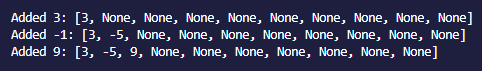
\includegraphics{Images/Testing/T3.8.1.PNG}
        \vspace{1cm}

        {\large Evidence 3.\rn } \\ 
        \vspace{0.3cm}
        Creating a Double Ended Queue with a length of 4, add Push Items to it, and get the 
        Items in First and Last \\

        \begin{minted}[frame=leftline,framesep=2mm,baselinestretch=1.2,fontsize=\footnotesize,linenos]{python}
deque = Deque(4)
deque.PushFront(3)
deque.PushFront(-5)
deque.PushFront(9)
deque.PushFront(4)
deque.PushFront(-4)

print("First:", deque.First())
print("Last:", deque.Last())
print("Queue:", deque.queue)
        \end{minted}

        The output of the above code: \\
        \includegraphics{Images/Testing/T3.9.PNG}
        \vspace{1cm}

        {\large Evidence 3.\rn } \\ 
        \vspace{0.3cm}
        Create a Double Ended Queue and Sample items from the Queue \\

        \begin{minted}[frame=leftline,framesep=2mm,baselinestretch=1.2,fontsize=\footnotesize,linenos]{python}
deque = Deque(4)
deque.PushFront(3)
deque.PushFront(-5)
deque.PushFront(9)
deque.PushFront(4)
deque.PushFront(-4)

print("Sample 1:", deque.Sample(2))
print("Sample 2:", deque.Sample(2))
print(deque.queue)
        \end{minted}

        The output of the above code: \\
        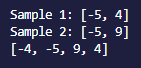
\includegraphics{Images/Testing/T3.10.1.PNG}
        \vspace{1cm}
    \end{center}

    \setcounter{magicrownumbers}{0}
    \begin{center}
        {\large Evidence 4.\rn } \\ 
        \vspace{0.3cm}

    \end{center}

    \setcounter{magicrownumbers}{0}
    \begin{center}
        {\large Evidence 5.\rn } \\ 
        \vspace{0.3cm}
        Randomnly Generated Unsorted List, sorted by the 1st Element to form the Sorted List \\

        \begin{minted}[frame=leftline,framesep=2mm,baselinestretch=1.2,fontsize=\footnotesize,linenos]{python}
inputList = [[random.randint(-10,10), random.randint(-10,10)] for i in range(5)]
print("Unsorted List:")
for item in inputList:
    print(item)

dl = DataCollector("SortingTest", [int, int], False)

dl.LogDataPointBatch(inputList)

sortedList = dl.HeapSort(0)

print("Sorted List:")
for item in sortedList:
    print(item)
        \end{minted}

        The output of the above code: \\
        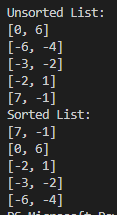
\includegraphics[width=3cm]{Images/Testing/T4.1.1.PNG} \\

        \vspace{1cm}

        {\large Evidence 5.\rn } \\ 
        \vspace{0.3cm}
        Adding a single point: [5, 2] to DataLogger \\
        \begin{minted}[frame=leftline,framesep=2mm,baselinestretch=1.2,fontsize=\footnotesize,linenos]{python}
dl = DataCollector("AddPointTest", [int, int], False)
print("Before: ", dl.dataPoints)

dl.LogDataPoint([5, 2])

print("After: ", dl.dataPoints)
        \end{minted}

        The output of the above code: \\
        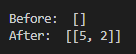
\includegraphics[width=4cm]{Images/Testing/T4.2.1.PNG} \\
        \vspace{1cm}

        {\large Evidence 5.\rn } \\ 
        \vspace{0.3cm}
        Test Data Point matches struture \\

        \begin{minted}[frame=leftline,framesep=2mm,baselinestretch=1.2,fontsize=\footnotesize,linenos]{python}
dl = DataCollector("Match Single Types", [int, float], False)

print("Matches Structure: ", dl.CheckMatchStructure([-3, 2.2]))
        \end{minted}

        The output of the above code: \\
        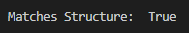
\includegraphics[width=4cm]{Images/Testing/T4.3.1.PNG} \\
        \vspace{1cm}

        {\large Evidence 5.\rn } \\ 
        \vspace{0.3cm}
        Test Data Point matches structure \\

        \begin{minted}[frame=leftline,framesep=2mm,baselinestretch=1.2,fontsize=\footnotesize,linenos]{python}
dl = DataCollector("Match Multi Typed", [bool, [float, int]], False)

print("Matches Structure: ", dl.CheckMatchStructure([False, 4.5]))
print("Matches Structure: ", dl.CheckMatchStructure([True, -9]))
        \end{minted}
            
        The output of the above code: \\
        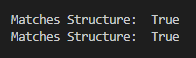
\includegraphics[width=4cm]{Images/Testing/T4.4.1.PNG} \\
        \vspace{1cm}

        {\large Evidence 5.\rn } \\ 
        \vspace{0.3cm}
        Test Data Point matches structure \\

        \begin{minted}[frame=leftline,framesep=2mm,baselinestretch=1.2,fontsize=\footnotesize,linenos]{python}
dl = DataCollector("Match List Type", [bool, str], False)

print("Matches Structure: ", dl.CheckMatchStructure([True, ["Matt", "Isabel", "Tristan", "Chris"]]))
        \end{minted}
                        
        The output of the above code: \\
        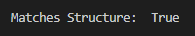
\includegraphics[width=4cm]{Images/Testing/T4.5.1.PNG} \\
        \vspace{1cm}

        {\large Evidence 5.\rn } \\ 
        \vspace{0.3cm}
        Test error thrown when Data Point doesnt match the given structure \\

        \begin{minted}[frame=leftline,framesep=2mm,baselinestretch=1.2,fontsize=\footnotesize,linenos]{python}
try:
    dl = DataCollector("Match Data Structure Error", [str, int], False)

    print("Matches Structure: ", dl.CheckMatchStructure(["Steve Preston", True]))
except Exception as x:
    print(x)
        \end{minted}

        The output of the above code: \\
        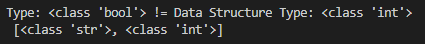
\includegraphics[width=8cm]{Images/Testing/T4.6.1.PNG} \\
        \vspace{1cm}

        {\large Evidence 5.\rn } \\ 
        \vspace{0.3cm}
        Select Prime numbers in 1st index\\

        \begin{minted}[frame=leftline,framesep=2mm,baselinestretch=1.2,fontsize=\footnotesize,linenos]{python}
inputList = [[random.randint(-10,10), random.randint(-10,10)] for i in range(5)]
print("Random List:")
for item in inputList:
    print(item)

dl = DataCollector("Select List", [int, int], False)

dl.LogDataPointBatch(inputList)

sortedList = dl.Select(0, [1,2,3,5,7])

print("Selected List:")
for item in sortedList:
    print(item)
        \end{minted}
            
        The output of the above code: \\
        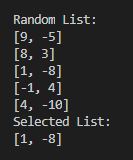
\includegraphics[width=3cm]{Images/Testing/T4.7.1.PNG} \\
        \vspace{1cm}

        {\large Evidence 5.\rn } \\ 
        \vspace{0.3cm}

        Test for saving a file \\
        \begin{minted}[frame=leftline,framesep=2mm,baselinestretch=1.2,fontsize=\footnotesize,linenos]{python}
inputList = [[random.randint(-10,10), random.randint(-10,10)] for i in range(5)]
print("Saved List:")
for item in inputList:
    print(item)

dl = DataCollector("Save-Load Test", [int, int], False)

dl.LogDataPointBatch(inputList)

dl.SaveDataPoints()
        \end{minted}

        The saved Data Points \\
        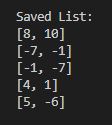
\includegraphics[width=3cm]{Images/Testing/T4.8.1.PNG} \\
        The saved file "Save-Load Test.data" \\
        
\includegraphics[width=4cm]{Images/Testing/T4.8.2.PNG} \\
        \vspace{1cm}

        {\large Evidence 5.\rn } \\ 
        \vspace{0.3cm}

        Test for loading a file
        \begin{minted}[frame=leftline,framesep=2mm,baselinestretch=1.2,fontsize=\footnotesize,linenos]{python}
dl = DataCollector("Save-Load Test", [int, int], True)

print("Loaded List:")
for item in dl.dataPoints:
    print(item)
        \end{minted}

        The File we're loading from "Save-Load Test.data" \\
        
\includegraphics[width=4cm]{Images/Testing/T4.8.2.PNG} \\
        The loaded Data Points \\
        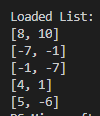
\includegraphics[width=3cm]{Images/Testing/T4.9.1.PNG} \\
        \vspace{1cm}
    \end{center}
   
\end{flushleft}